\chapter{Experiments}\label{chap:experiments}

\section{Settings}
\subsection{Libraries}\label{pypsa}
A key role for the implementation plays \textit{PyPSA} (Python for Power System Analysis) \cite{brown2017pypsa}, which is a toolbox to simulate and optimize power systems. The components of its network container are very closely related to the network components presented in section \ref{sec:components}. \textit{PyPSA's} Buses are the fundamental nodes to which all loads, generators, lines and transformers attach. According to Kirchhoff's current law everything feeding in out of the buses is balanced out to enforce energy conservation. The data is stored in \textit{pandas} DataFrames to enable efficient calculations. \textit{PyPSA} is also able to perform a power flow analysis on the network, which is important for the calculation of the penalty term among other functionalities. \textit{Networkx} is used by the algorithm to store and modify the graph which represents the electric grid.

\subsection{Example Grid}
For testing and evaluating the algorithm the grid of a village in rural Germany is used (exact name and location is omitted due to data protection). It is a mixed grid which consists of a medium and low voltage level. It connects to the higher voltage level from the south (cut off). It consists of 1857 buses, 1851 lines, 16 MV/LV transformer stations which connect the medium voltage level to the underlying low voltage level and 1 HV/MV transformer which connects the whole network to the upstream high voltage grid. \\
Although the network contains only 17 transformers, the number of possible rings, which connect the transformers is very large ($\frac{17!}{2} \approx 1.77*10^{14}$ [number of permutations divided by two, since the exact reverse order of stations is considered the same ring]). \\
\begin{figure}[h]
	\begin{centering}
		{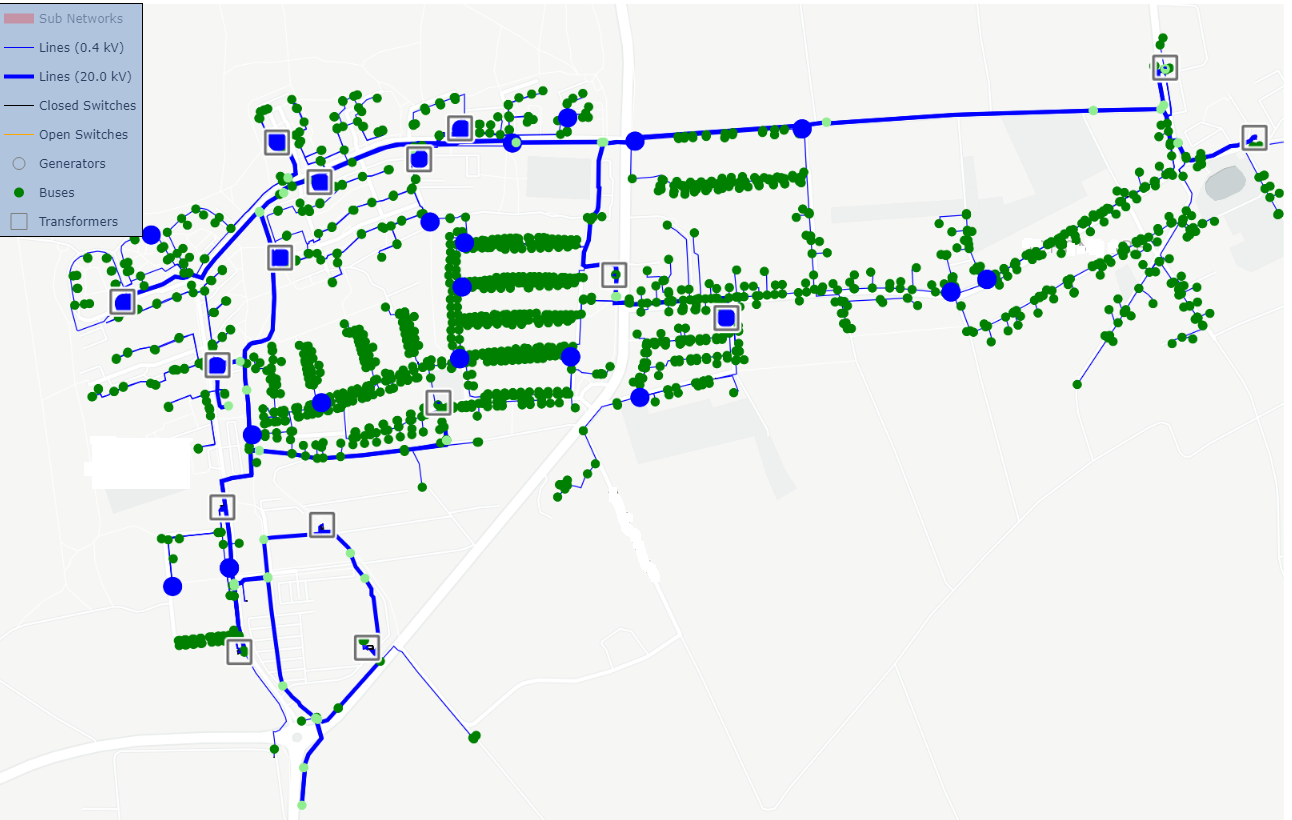
\includegraphics[scale=0.5]{figures/experiments/enwg_mixed.png}}
		\caption{The grid used for testing. (internally developed tool used for visualization)}
		\label{fig:enwg_mixed}
	\end{centering}
\end{figure}

\subsection{Grid Extraction}\label{sec:extraction}
The algorithm was specifically designed for the medium voltage level and therefore the input grid needs to fulfill the following requirements:
\begin{itemize}
	\setlength\itemsep{-1em}
	\item The input grid should contain only medium voltage buses (20 kV)
	\item All buses must have coordinates (for the triangulation)
	\item The buses loads are an aggregation of the loads of the underlying LV grid.
	\item The input grid only contains MV transmission lines (20 kV)
	\item The lines always directly connect two buses. 
	\item There has to exist at least one HV/MV transformer from where the algorithm can start.
\end{itemize}

\begin{figure}[h]
	\begin{centering}
		{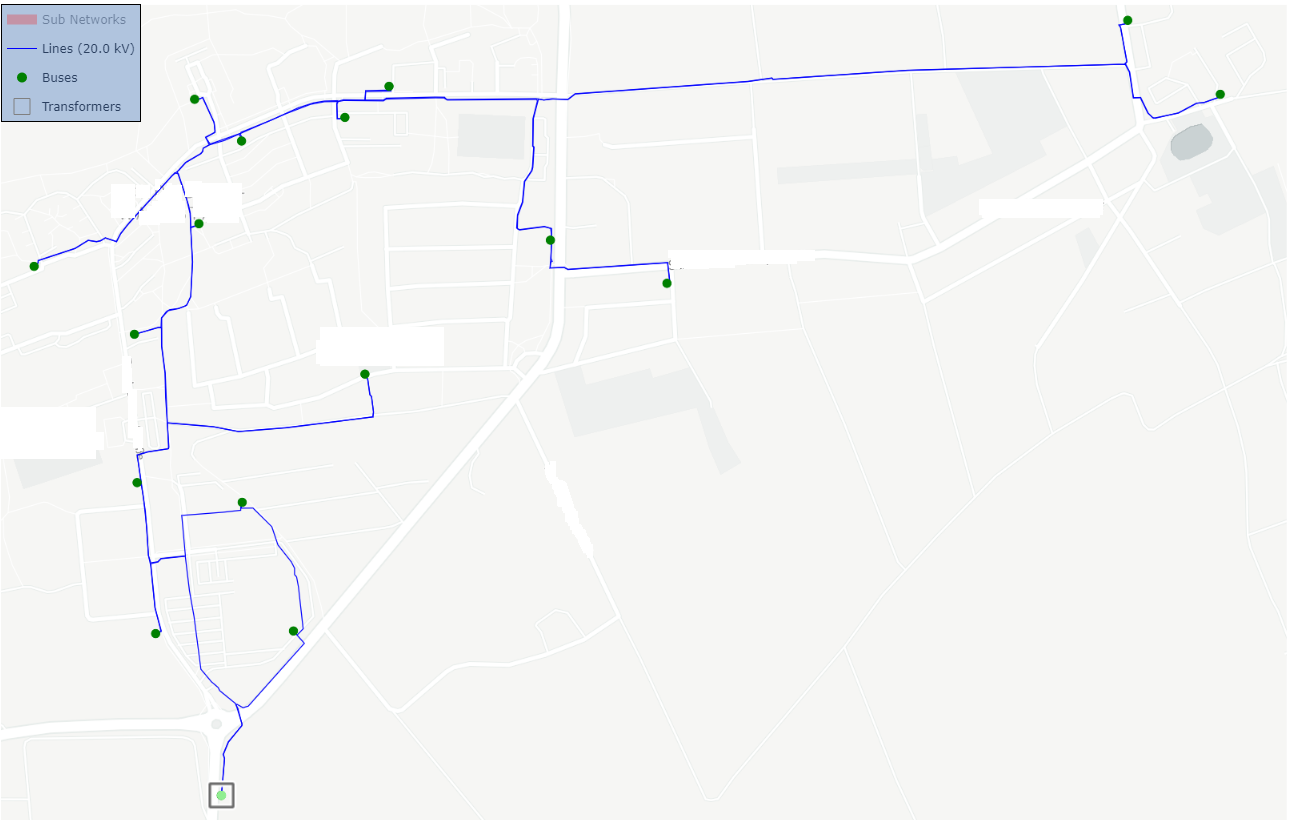
\includegraphics[scale=0.5]{figures/experiments/enwg_mv.png}}
		\caption{Middle voltage part of the grid.}
		\label{fig:enwg_mv}
	\end{centering}
\end{figure}


In a preprocessing step the MV part of the original grid is extracted (see Figure \ref{fig:enwg_mv}), to bring the input of the algorithm in the required form. After the extraction only the MV buses of the transformers are kept (in \textit{PyPSA} transformers connect two buses of different voltages). The task of the algorithm is to connect the buses via transmission lines in the most cost effective way, while satisfying the given side constraints. The blue lines are MV cables which already exist in the network and which can be used by the algorithm at zero cost. The green dots resemble the buses.



\begin{figure}[h]
	\begin{centering}
		{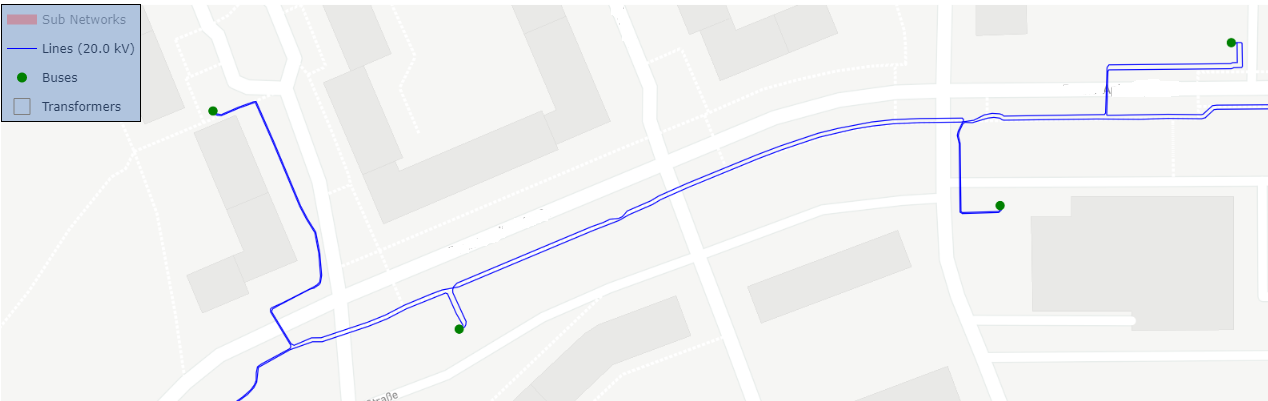
\includegraphics[scale=0.5]{figures/experiments/enwg_zoom.png}}
		\caption[Example graph zoom]{Parallel lines in the ring of the MV grid.}
		\label{fig:enwg_zoom}
	\end{centering}
\end{figure}

At first glance, the topology of the extracted MV grid does not look like it possesses the required ring structure. Only when zoomed in it is possible to see, that through parallel lines, the ring structure is maintained (see Figure \ref{fig:enwg_zoom}). It is debatable however, whether is it useful to put two lines in parallel to achieve adequate security. More to this in the discussion section \ref{sec:discussion}.


%\begin{figure}[h]
	\begin{centering}
		{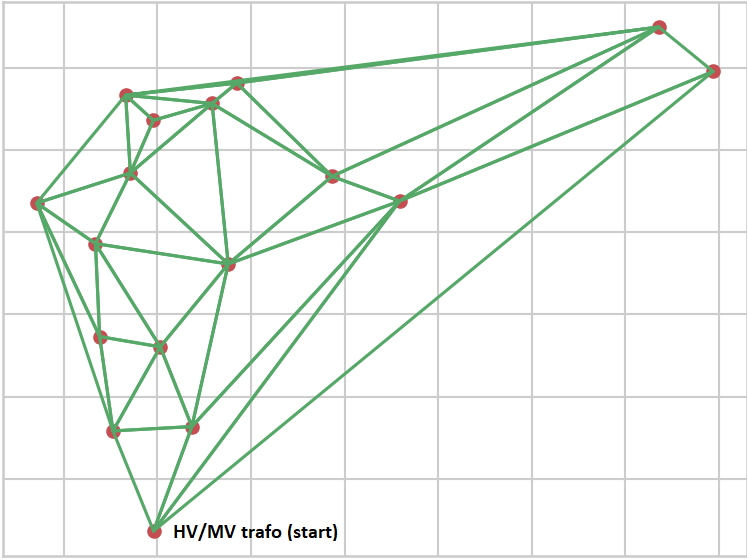
\includegraphics[scale=0.5]{figures/experiments/1000_iter/tri_1000.png}}
		\caption{Triangulation of the MV grid.}
		\label{fig:tri_1000}
	\end{centering}
\end{figure}


\begin{figure}
	\centering
	\begin{minipage}{.5\textwidth}
		\centering
		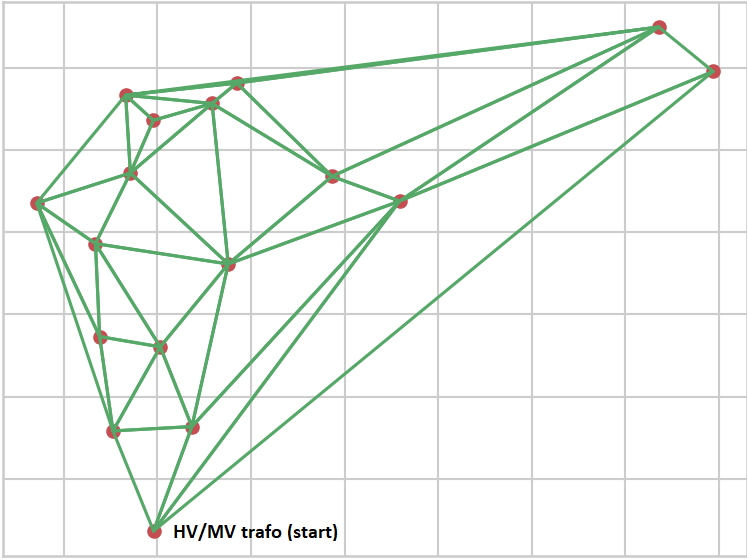
\includegraphics[width=.9\linewidth]{figures/experiments/1000_iter/tri_1000.png}
		\captionof{figure}{Triangulation.}
		\label{fig:tri_1000}
	\end{minipage}%
	\begin{minipage}{.5\textwidth}
		\centering
		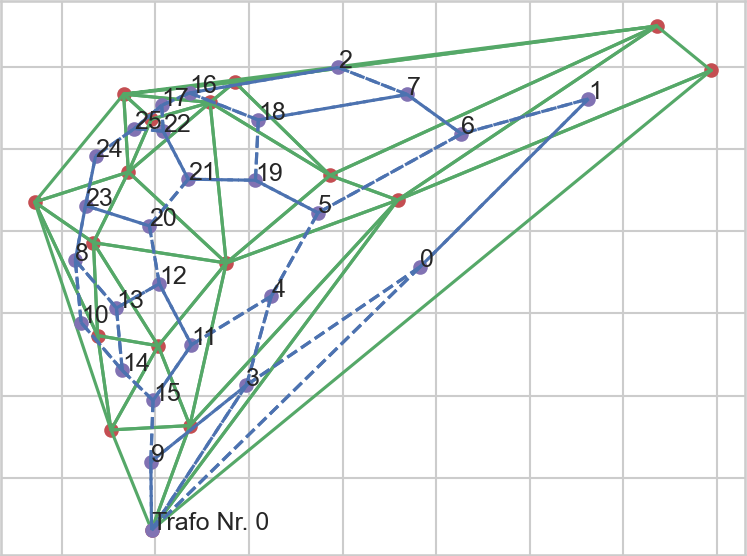
\includegraphics[width=.9\linewidth]{figures/experiments/1000_iter/tri_ant_1000.png}
		\captionof{figure}{Ant graph.}
		\label{fig:tri_ant_1000}
	\end{minipage}
\end{figure}

 %(green) and ant graph (blue) of the MV grid.
In Figure \ref{fig:tri_1000} the triangulation of the buses of the MV grid is shown in a schematic view. From the triangulation, the ant graph is built. Figure \ref{fig:tri_ant_1000} shows the associated ant graph. The blue ant nodes are the incenter of the triangles. Neighboring ant nodes are connected via an edge (dotted lines do not have a specific meaning in this context).

%\begin{figure}[h]
	\begin{centering}
		{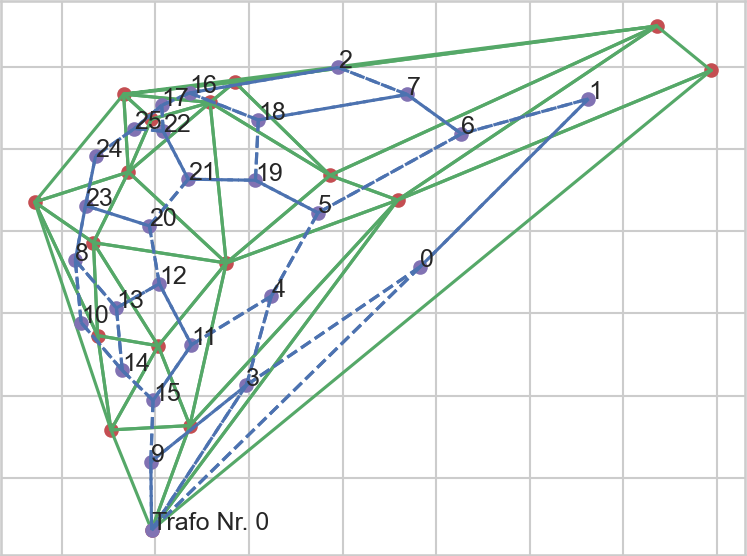
\includegraphics[scale=0.5]{figures/experiments/1000_iter/tri_ant_1000.png}}
		\caption{Triangulation (green) and ant graph (blue) of the MV grid.}
		\label{fig:tri_ant_1000}
	\end{centering}
\end{figure}


\section{Results}

\begin{figure}[h]
	\begin{centering}
		{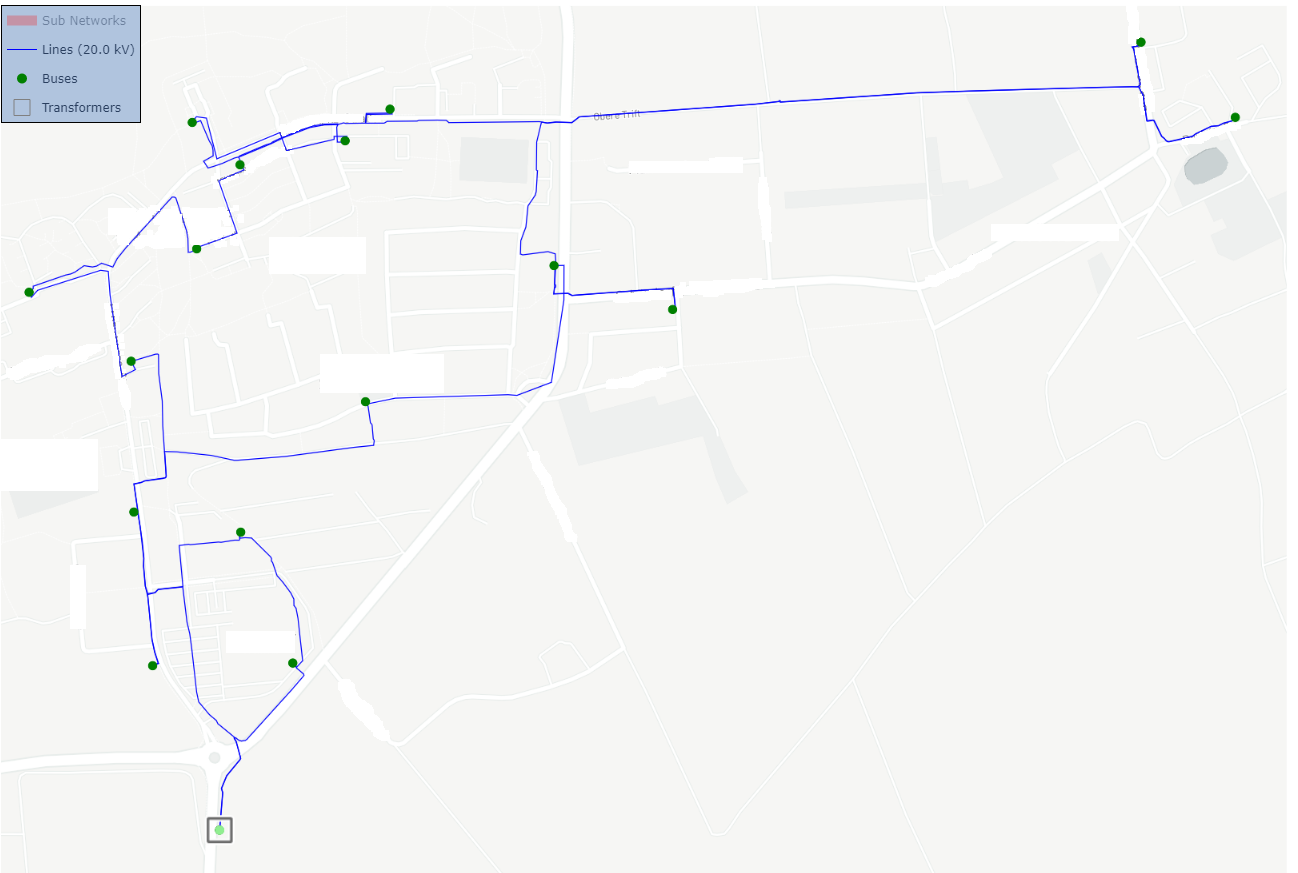
\includegraphics[scale=0.5]{figures/experiments/1000_iter/pypsa_1000.png}}
		\caption{Result network of best found MV grid.}
		\label{fig:pypsa_1000}
	\end{centering}
\end{figure}


The best result found by APMV is shown in Figure \ref{fig:pypsa_1000}. Most of the lines which are used in the input grid are also part of the result grid since they can be reused at zero cost. Four lines are new and added by the algorithm alongside streets. The penalty term for electric constraint violation is kept to zero.

\begin{figure}[h]
	\begin{centering}
		{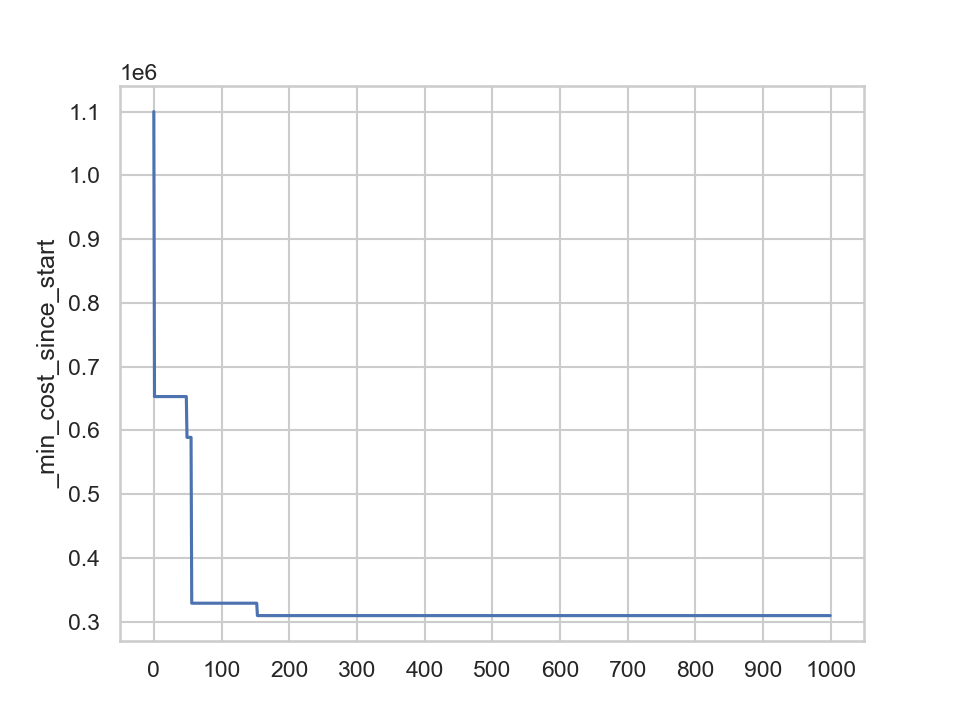
\includegraphics[scale=0.6]{figures/experiments/1000_iter/min_cost_1000.png}}
		\caption[Minimal cost]{Minimal cost found since the start.}
		\label{fig:min_cost_1000}
	\end{centering}
\end{figure}


The associated costs are depicted in Figure \ref{fig:min_cost_1000}. The minimal cost found by the algorithm declines rapidly in the first iterations and then plateaus out after a small drop at around iteration 150. This last decrease in cost was not captured by other runs, since they were capped at 100 iterations. The step-wise decrease in cost is due to a new and cheaper routing being found (drop) after which the algorithm produces only equal or worse solutions (plateau). Important to notice, is that the minimal found cost of ca. 309.000 Euro does not reflect the total cost of the network, but only the lines additionally built by the algorithm. Already existing lines do not appear in the cost function since their cost is zero. To calculate the total cost of the solution including the existing lines, all lines were considered to be newly built by the algorithm in a post processing step. This lead to a cost of 1.95M Euro. This cost can now be compared to the same calculation done with the extracted MV grid of the input. This results in costs of 2.17M Euros. The found solution of the algorithm is therefore only 89\% of the cost of the input grid.



\begin{figure}[h]
	\begin{centering}
		{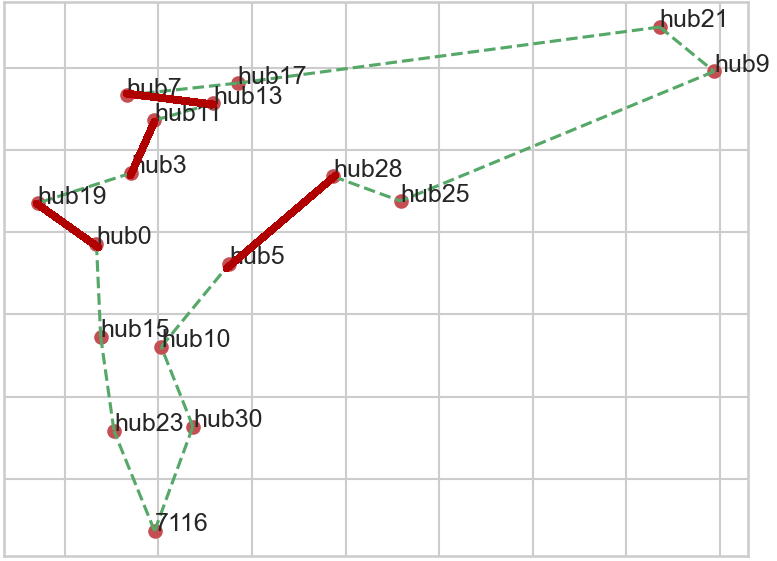
\includegraphics[scale=0.6]{figures/experiments/1000_iter/best_mv_1000.png}}
		\caption[Result grid schematic]{Schematic view of the best found MV grid. The "hubs" resemble MV/LV trafos which need to be connected to "7116" - the HV/MV trafo. Newly created lines by the algorithm are marked red.}
		\label{fig:best_mv_1000}
	\end{centering}
\end{figure}


To better see how the algorithm connects the buses a schematic view of the solution is given in Figure \ref{fig:best_mv_1000}. Here the rings structure is clearly visible. 





\subsection{Parameterstudy}
As listed in section \ref{parameters}, the algorithm has fairly many input parameters. Trying out multiple values for each parameter in all possible combinations would therefore be unfeasible. Instead, single parameters are are varied while the remaining parameters are kept at their default values. When only single parameters are varied, interactions between parameters can unfortunately not be traced anymore. \\

The parameter study is divided into four parts. First, the parameter for maximum number of stations per ring is studied (maximalRingsize). The second part investigates the parameter that changes the number of constructed solutions (antsPerColony, iterations). The third part examines the parameter controlling the expansion rule ($q0$, $\alpha$, $\beta$) and the last part studies the parameter controlling the pheromone update ($\rho$, $\xi$).

\subsubsection{Control Maximum Number of Stations per Ring}\label{stations_per_ring}
In the first part the maximal number of buses per ring are limited to a fixed value. Limiting the number of stations per ring can be useful to reduce the loading of the lines due to a smaller number of connected loads. Additionally, it decrease the number of stations being cut off electricity in case of a failure. Limiting the number of stations can be done easily during the expansion process of the ant. When an ant expands a new triangle during the solution building process, the number of stations of the ring also increases by one (neighboring triangles already share two corners). This applies to all triangles except the very first one expanded from the HV/MV transformer, where two stations are added. The number of stations per ring is therefore the number of expanded triangles incremented by one. When the ant reaches the maximum number of triangles it is allowed to expand, it stops with the expansion and starts constructing a new ring starting from the HV/MV trafo. Downwards, the maximal number of stations per ring is limited depending on the structure of the grid. The smallest number of stations per ring for which the algorithm was able to find a solution is eight. For less then eight stations per ring it is impossible to build a solution, due to the problem formulated in section \ref{sec:tri_problem}. There exist only three neighboring triangles to the start transformer and each ring occupies at least one of them. If all neighbors of the start transformer are blocked but some stations are still not connected, the ant must perform a restart. In case of maximal seven stations per ring, the ant restarted every solution building attempt out of 1500. A Manual check confirmed that it is indeed impossible for the algorithm ti find a solution.


\begin{figure}
	\centering
	\begin{minipage}{.5\textwidth}
		\centering
		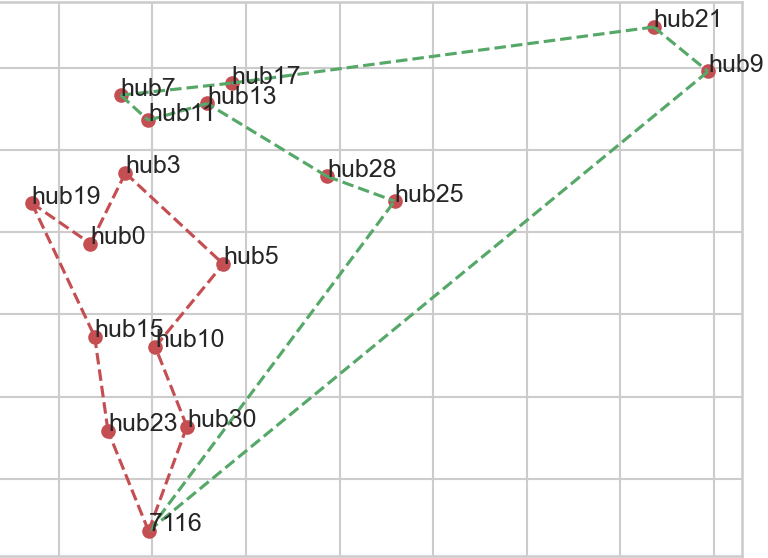
\includegraphics[width=1\linewidth]{figures/experiments/ringsize/size_8_9.png}
		\captionof{figure}[Max. 8/9 buses per ring schematic]{Max. 8/9 buses per ring.}
		\label{fig:ringsize_89}
	\end{minipage}%
	\begin{minipage}{.5\textwidth}
		\centering
		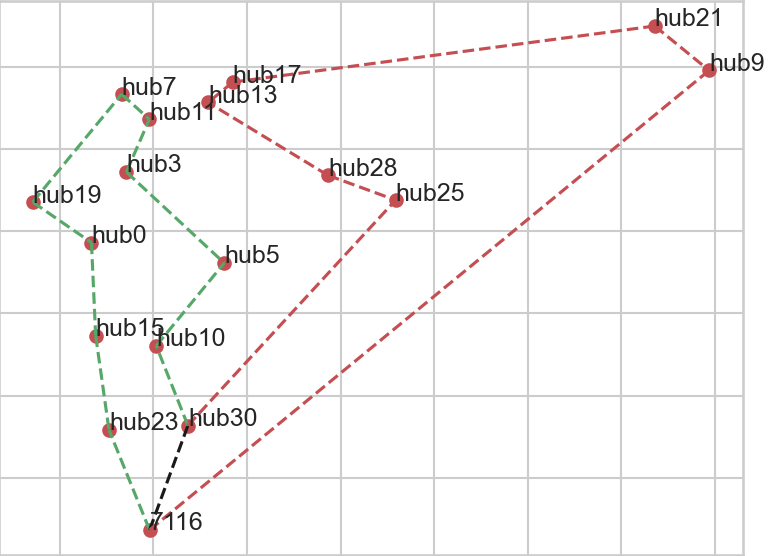
\includegraphics[width=1\linewidth]{figures/experiments/ringsize/size_10.png}
		\captionof{figure}[Max. 10 buses per ring schematic]{Max. 10 buses per ring.}
		\label{fig:ringsize_10}
	\end{minipage}
\end{figure}
Figure \ref{fig:ringsize_89} and \ref{fig:ringsize_10} show the rings being build when limiting the maximum number of stations to 8,9 and 10 in the schematic view of the map (they both can be seen in the appendix with the actual course of lines). The predicted cost of building the network as suggested in Figure \ref{fig:ringsize_89} would amount to 2.53M Euro (117 \% when compared to te original network) and 2.52M Euro (116 \%) for the network suggested in Figure \ref{fig:ringsize_10}. In general it makes sense, that increasing the number of rings also increase the cost, since additional cables are required to return to the HV/MV transformer. For more than 10 but less than 16 stations the algorithm found the same solution as shown in Figure \ref{fig:ringsize_10} and for 16 or more stations the algorithm suggested building a single ring, which is the cheapest option for this grid.

%\begin{figure}[h]
	\begin{centering}
		{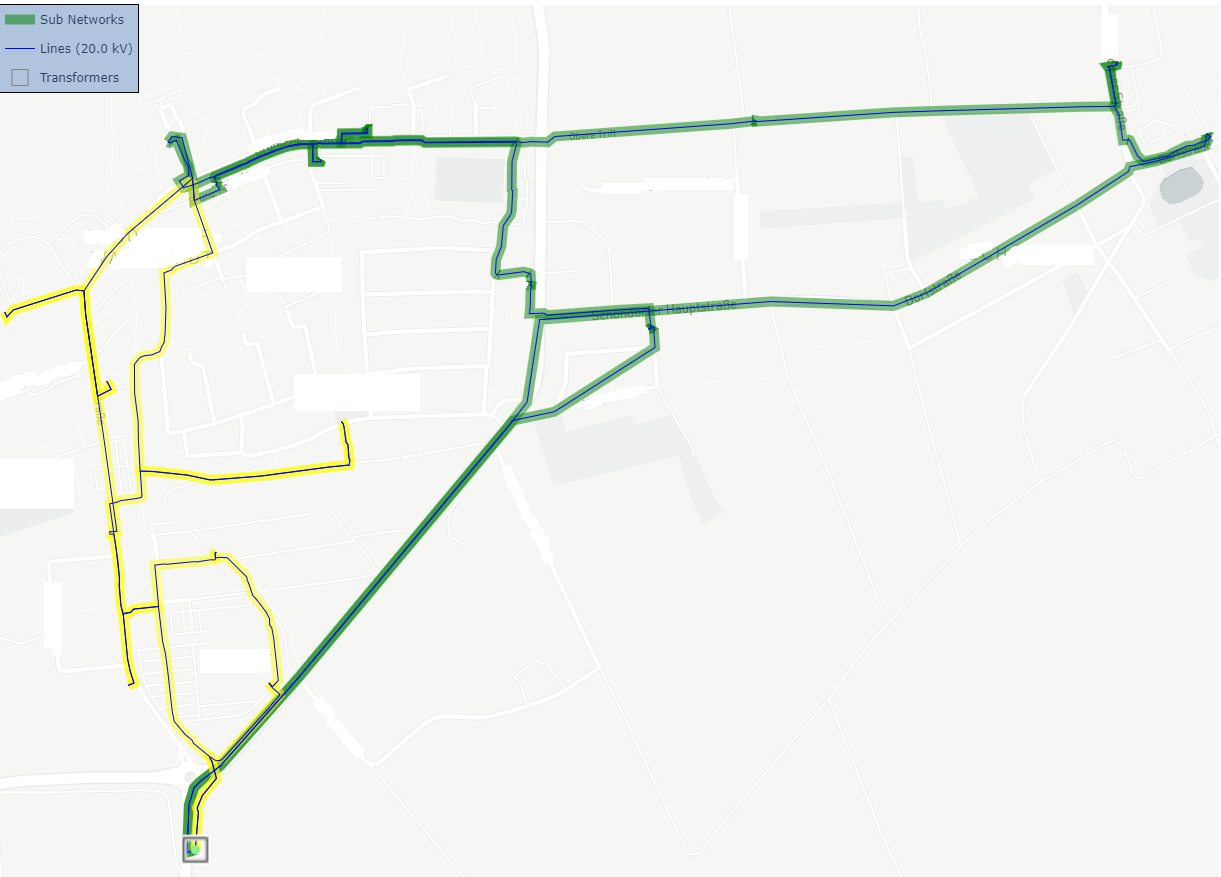
\includegraphics[scale=0.4]{figures/experiments/ringsize/ringsize89_2.png}}
		\caption{Max. 8/9 buses per ring (MV)}
		\label{fig:ringsize89_2}
	\end{centering}
\end{figure}

%\begin{figure}[h]
	\begin{centering}
		{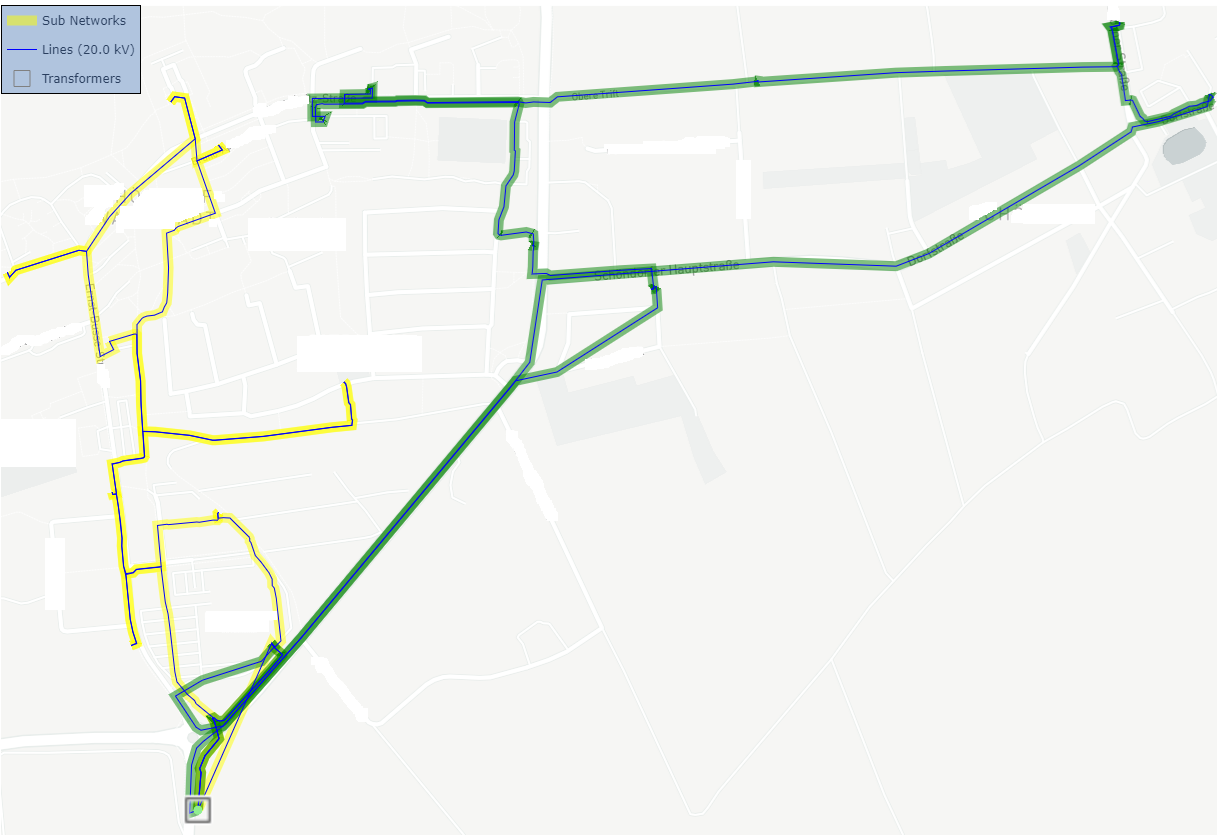
\includegraphics[scale=0.4]{figures/experiments/ringsize/ringsize10_2.png}}
		\caption{Max. ten buses per ring (MV)}
		\label{fig:ringsize10_2}
	\end{centering}
\end{figure}

%\begin{figure}[h]
	\begin{centering}
		{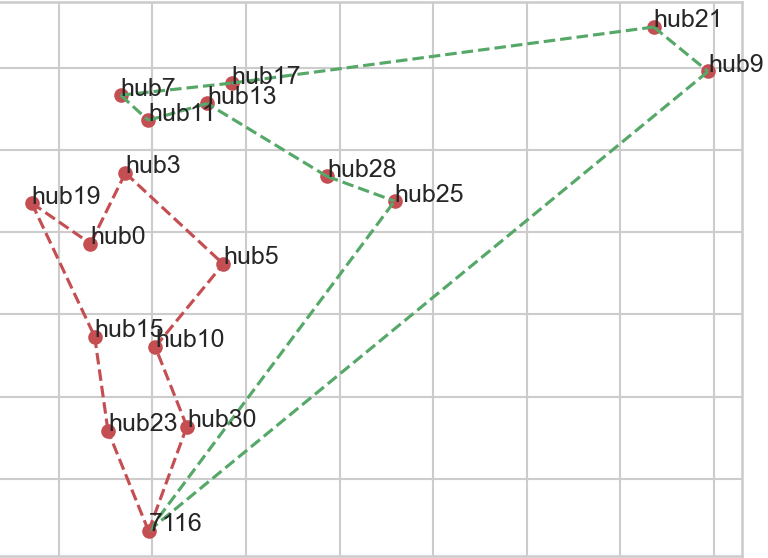
\includegraphics[scale=0.7]{figures/experiments/ringsize/size_8_9.png}}
		\caption{Schematic view of the best found MV grid with a maximum of eight or nine stations per ring.}
		\label{fig:ringsize_8_9}
	\end{centering}
\end{figure}

%\begin{figure}[h]
	\begin{centering}
		{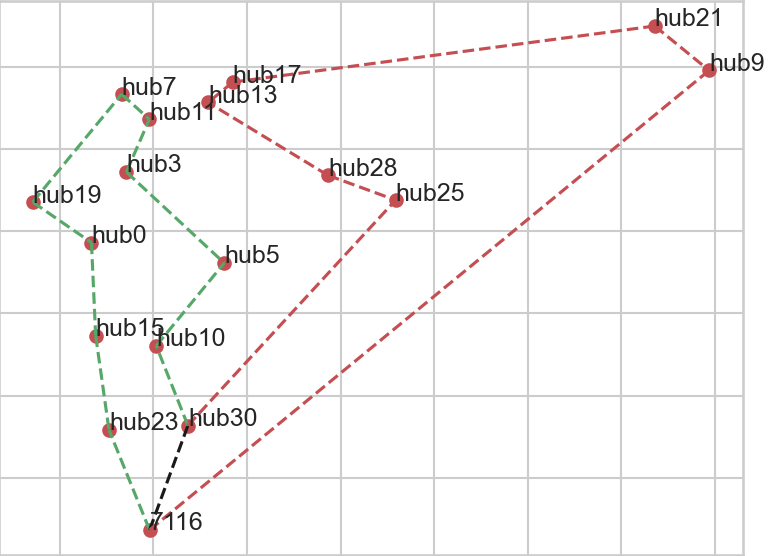
\includegraphics[scale=0.7]{figures/experiments/ringsize/size_10.png}}
		\caption{Schematic view of the best found MV grid with a maximum of ten stations per ring.}
		\label{fig:ringsize_10}
	\end{centering}
\end{figure}


\subsubsection{Control Number of Constructed Solutions}\label{constructed_solutions}

To perform well, ACO algorithms need to learn from previous iterations and explore a sufficient area of the search space. Even though the heuristic function can lead ants quickly towards reasonable results the number of constructed solutions plays a major role. \textit{Ant-Colony-System} \cite{ant_coloy_system} by Dorigo et. al. presents three parameters to control the number of constructed solutions. The number of iterations, the number of colonies and the number of ants per colony. The ants solution building process is only dependent on the best solution of the previous iteration and not on the solutions built by other ants in the same iteration. Therefore, a second independent colony of ants could create a solution in parallel. \textit{APMV} is a sequential algorithm therefore the number of colonies is always set to one. In future work the feature of multiple colonies per iteration could be added to reduce runtime. \\
How the minimal found cost change with respect to the number of iterations can already be seen in Figure \ref{fig:min_cost_1000}. On this test grid the greatest reduction in cost is already achieved after ca. 50 iterations. Around iteration 150 another small decrease in cost can be observed. Due to limited computational resources though, the default number of iterations is set to 100. An automated stop of searching for a further decrease in cost after a certain amount of iterations could be implemented.
\begin{figure}[h]
	\begin{centering}
		{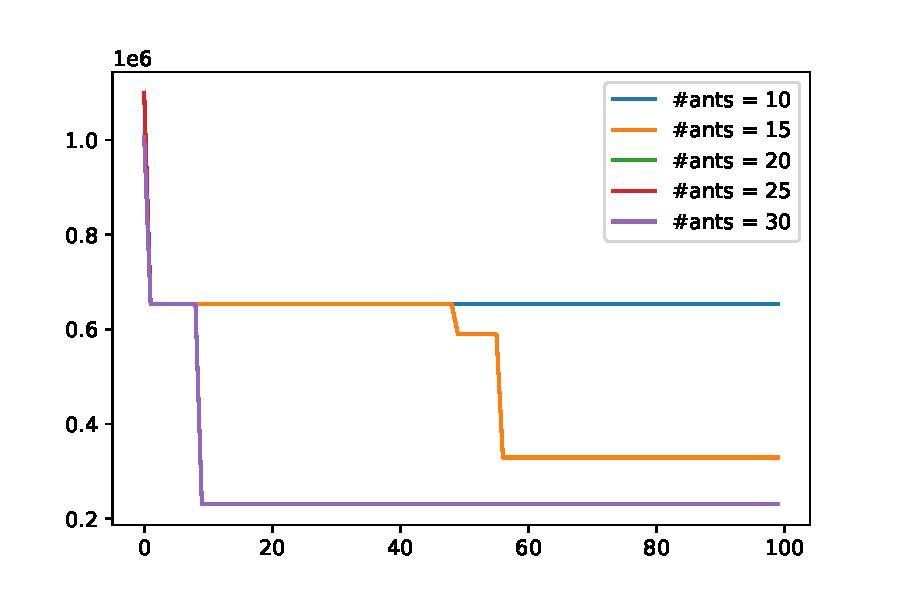
\includegraphics[scale=0.7]{figures/experiments/plt_ant.pdf}}
		\caption[Parameter study: number of ants]{Minimal cost found since the start for different number of ants per iteration.}
		\label{fig:plt_ant}
	\end{centering}
\end{figure}

The number of ants per iteration is the third parameter to control the number of constructed solutions. Its effect is shown in Figure \ref{fig:plt_ant}, which depicts the minimum cost found for different number of ants per iteration. The cost for 20 and 25 ants per iteration is congruent with the cost for 30 ants per iteration (this might be caused by the usage of the same seed in the algorithms random functions). For 20,25 and 30 ants the algorithm yields the best results. Using less ants per iteration might lead to less exploration and therefore a convergence towards a local minimum. In the future it would be interesting to increase the number of ants even further until the performance would decline again.

\subsubsection{Control Expansion Rule}\label{expansion_rule}
The parameters which control the expansion rule are $q0$, $\alpha$ and $\beta$. They guide the ant in its decision which node to expand next. The parameter $q0$ determines to which extend the ant is influenced by knowledge of the best solution of previous iterations. It modulates the trade-off between exploitation and exploration. Figure \ref{fig:q_0} shows the minimal cost found at a certain iteration with respect to different values of $q0$. For $q0 = 1$ the ant builds a solution and is forced afterwards to always expand the exact same components since no exploration is allowed. That is why the ant can never explore a better solution and therefore the costs can never decrease. The best solution is found for $q0 = 0.75$, since it enables the ant to explore more of the search space. Similar to the number of ants in the previous subsection it would interesting to investigate even lower values for $q0$ in the future until the performance of the algorithm would decline again. \\
\begin{figure}[h]
	\begin{centering}
		{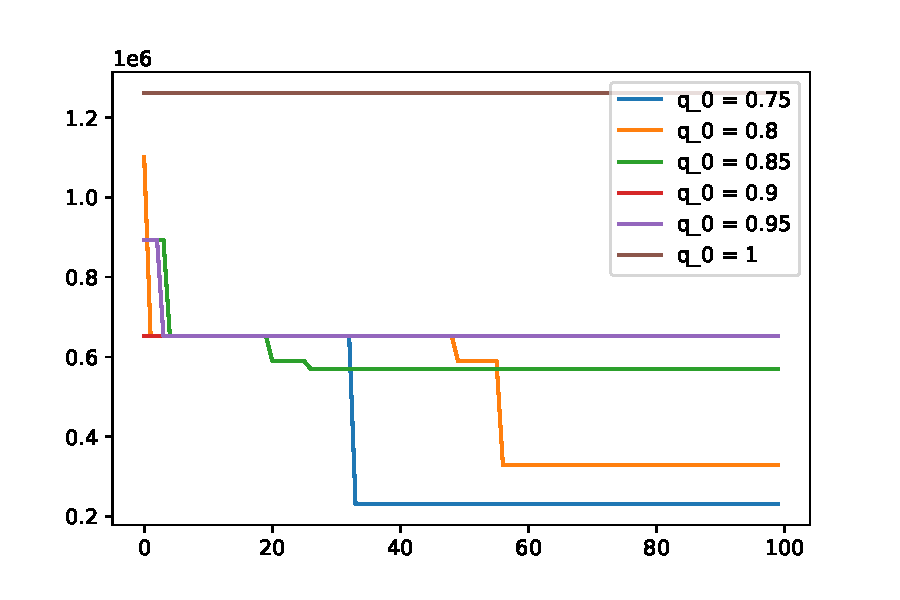
\includegraphics[scale=0.8]{figures/experiments/q_0.pdf}}
		\caption[Parameter study: $\protect q0$]{Minimal cost found since the start for different $\protect q0$.}
		\label{fig:q_0}
	\end{centering}
\end{figure}

The parameters $\alpha$ and $\beta$ describe how much the ants decision process of expanding new nodes should be guided by pheromones or heuristics.

\begin{figure}[h]
	\begin{centering}
		{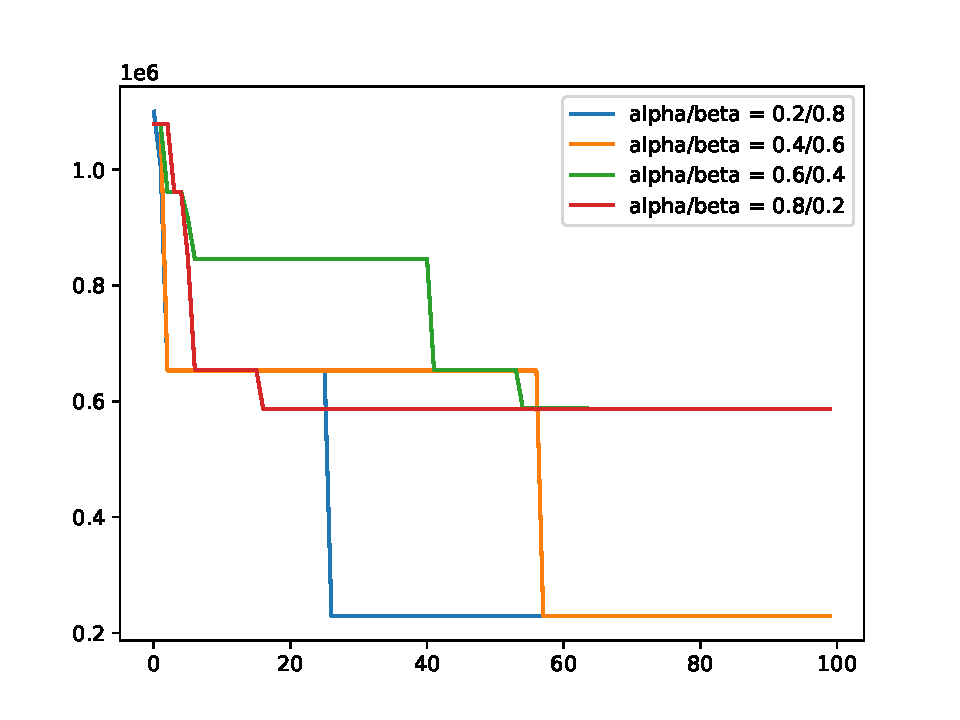
\includegraphics[scale=0.8]{figures/experiments/alpha_beta.pdf}}
		\caption{Minimal cost found since the start for different configurations of $\protect\alpha$ and $\protect\beta$.}
		\label{fig:alpha_beta}
	\end{centering}
\end{figure}

\subsubsection{Control Pheromone Update}\label{pheromone_update}

Results of different estimated min cost:
	- looks like as long as emec cost is lower than real cost the convergence is good!

\subsection{Runtime}
\subsection{Discussion}\label{sec:discussion}
\subsubsection{Triangulation and Parallel Lines}
	- kann eigentlich keine parallelen ringe. (diese sind aber anscheinend in Nutzung)
	- bessere Sicherheit ohne parallele lines?